\documentclass[aspectratio=169]{beamer}
%\usepackage[english,greek]{babel}
%\usepackage[iso-8859-7]{inputenc}
\usepackage{euler}
\usepackage{graphicx,pgfplots,tikz}

\beamertemplatenavigationsymbolsempty

\begin{document}
	\begin{frame}{$k=1$}
		\begin{figure}
			\resizebox{\linewidth}{!}{\begin{tikzpicture}
			\draw[thick,->] (-.5,0) -- (6,0);
			\draw[thick,->] (0,-1.5) -- (0,1.5);
			\draw[blue, domain={0.01}:{5.8}, samples=200] plot (\x,{sin(\x r)});
			\end{tikzpicture}}
		\end{figure}
	\end{frame}

\begin{frame}{$k=1.5$}
	\begin{figure}
		\resizebox{\linewidth}{!}{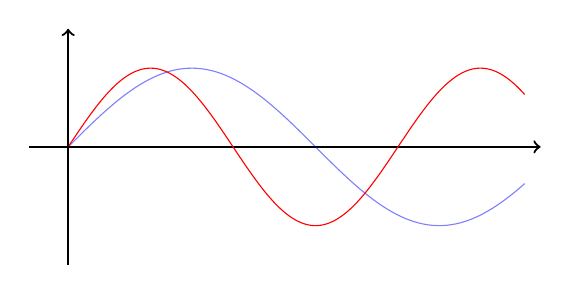
\begin{tikzpicture}
			\draw[thick,->] (-.5,0) -- (6,0);
			\draw[thick,->] (0,-1.5) -- (0,1.5);
			\draw[blue, opacity=.5, domain={0.01}:{5.8}, samples=100] plot (\x,{sin(\x r)});
			\draw[red, domain={0.01}:{5.8}, samples=200] plot (\x,{sin(1.5*\x r)});
			\end{tikzpicture}}
	\end{figure}
\end{frame}

\begin{frame}{$k=2$}
	\begin{figure}
		\resizebox{\linewidth}{!}{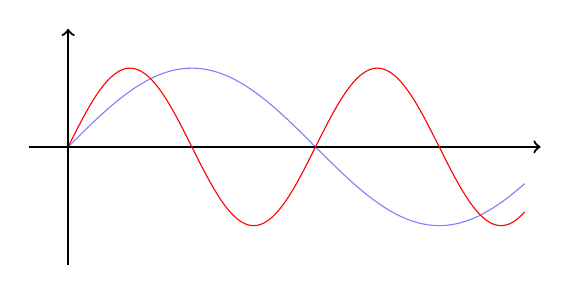
\begin{tikzpicture}
			\draw[thick,->] (-.5,0) -- (6,0);
			\draw[thick,->] (0,-1.5) -- (0,1.5);
			\draw[blue, opacity=.5, domain={0.01}:{5.8}, samples=100] plot (\x,{sin(\x r)});
			\draw[red, domain={0.01}:{5.8}, samples=200] plot (\x,{sin(2*\x r)});
			\end{tikzpicture}}
	\end{figure}
\end{frame}

\begin{frame}{$k=2.5$}
	\begin{figure}
		\resizebox{\linewidth}{!}{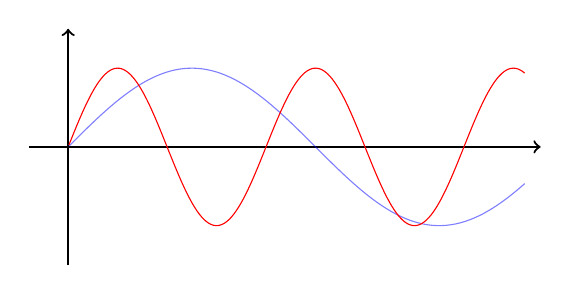
\begin{tikzpicture}
			\draw[thick,->] (-.5,0) -- (6,0);
			\draw[thick,->] (0,-1.5) -- (0,1.5);
			\draw[blue, opacity=.5, domain={0.01}:{5.8}, samples=100] plot (\x,{sin(\x r)});
			\draw[red, domain={0.01}:{5.8}, samples=200] plot (\x,{sin(2.5*\x r)});
			\end{tikzpicture}}
	\end{figure}
\end{frame}

\begin{frame}{$k=3$}
	\begin{figure}
		\resizebox{\linewidth}{!}{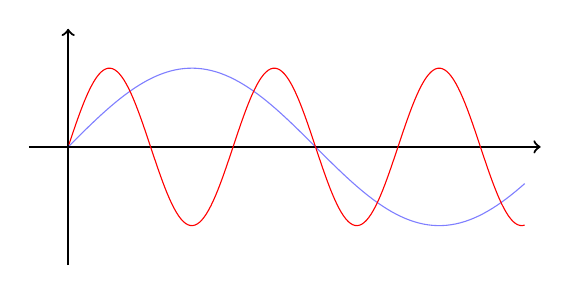
\begin{tikzpicture}
			\draw[thick,->] (-.5,0) -- (6,0);
			\draw[thick,->] (0,-1.5) -- (0,1.5);
			\draw[blue, opacity=.5, domain={0.01}:{5.8}, samples=100] plot (\x,{sin(\x r)});
			\draw[red, domain={0.01}:{5.8}, samples=200] plot (\x,{sin(3*\x r)});
			\end{tikzpicture}}
	\end{figure}
\end{frame}

\begin{frame}{$k=3.5$}
	\begin{figure}
		\resizebox{\linewidth}{!}{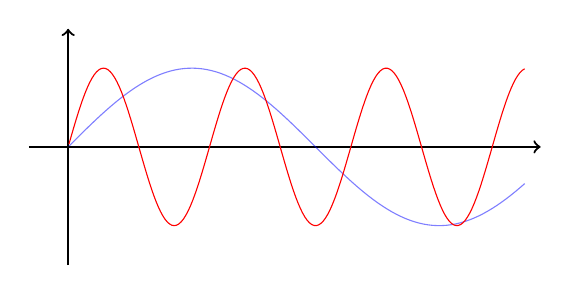
\begin{tikzpicture}
			\draw[thick,->] (-.5,0) -- (6,0);
			\draw[thick,->] (0,-1.5) -- (0,1.5);
			\draw[blue, opacity=.5, domain={0.01}:{5.8}, samples=100] plot (\x,{sin(\x r)});
			\draw[red, domain={0.01}:{5.8}, samples=200] plot (\x,{sin(3.5*\x r)});
			\end{tikzpicture}}
	\end{figure}
\end{frame}

\begin{frame}{$k=4$}
	\begin{figure}
		\resizebox{\linewidth}{!}{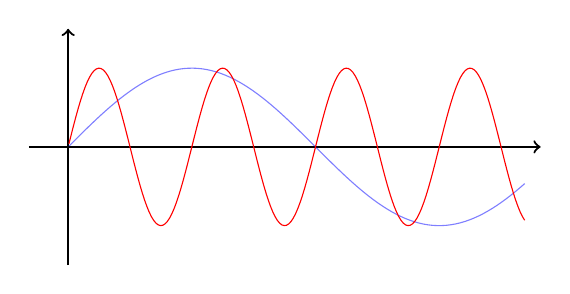
\begin{tikzpicture}
			\draw[thick,->] (-.5,0) -- (6,0);
			\draw[thick,->] (0,-1.5) -- (0,1.5);
			\draw[blue, opacity=.5, domain={0.01}:{5.8}, samples=100] plot (\x,{sin(\x r)});
			\draw[red, domain={0.01}:{5.8}, samples=200] plot (\x,{sin(4*\x r)});
			\end{tikzpicture}}
	\end{figure}
\end{frame}

\begin{frame}{$k=4.5$}
	\begin{figure}
		\resizebox{\linewidth}{!}{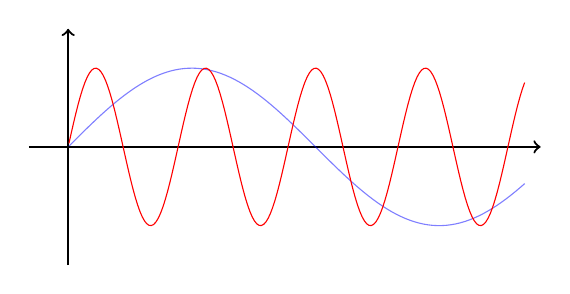
\begin{tikzpicture}
			\draw[thick,->] (-.5,0) -- (6,0);
			\draw[thick,->] (0,-1.5) -- (0,1.5);
			\draw[blue, opacity=.5, domain={0.01}:{5.8}, samples=100] plot (\x,{sin(\x r)});
			\draw[red, domain={0.01}:{5.8}, samples=200] plot (\x,{sin(4.5*\x r)});
			\end{tikzpicture}}
	\end{figure}
\end{frame}

\begin{frame}{$k=5$}
	\begin{figure}
		\resizebox{\linewidth}{!}{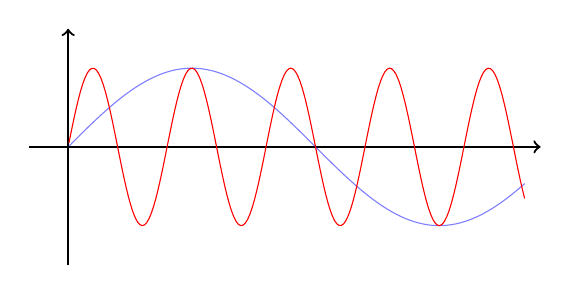
\begin{tikzpicture}
			\draw[thick,->] (-.5,0) -- (6,0);
			\draw[thick,->] (0,-1.5) -- (0,1.5);
			\draw[blue, opacity=.5, domain={0.01}:{5.8}, samples=100] plot (\x,{sin(\x r)});
			\draw[red, domain={0.01}:{5.8}, samples=200] plot (\x,{sin(5*\x r)});
			\end{tikzpicture}}
	\end{figure}
\end{frame}
\end{document}